\documentclass[border=10pt]{standalone}
\usepackage{tikz}
\usetikzlibrary{arrows.meta, positioning, calc, decorations.pathreplacing, fit}
\usepackage{amsmath, amssymb}

% Colors
\definecolor{bpgreen}{RGB}{80,170,100}
\definecolor{bplight}{RGB}{200,235,200}
\definecolor{gnnblue}{RGB}{90,140,200}
\definecolor{gnnlight}{RGB}{200,220,245}
\definecolor{filmred}{RGB}{200,75,60}
\definecolor{filmlight}{RGB}{250,225,220}
\definecolor{gy}{RGB}{105,105,105}
\definecolor{synred}{RGB}{180,60,50}

\begin{document}
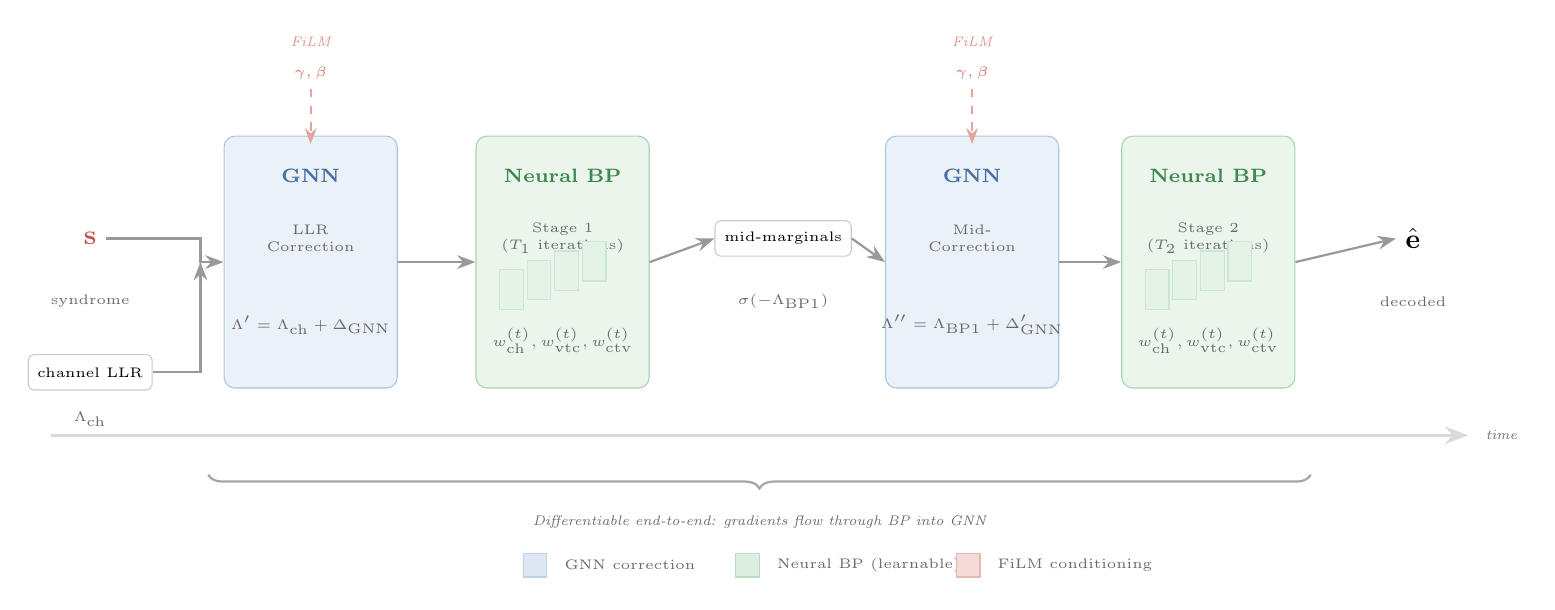
\begin{tikzpicture}[>=Stealth, font=\sffamily,
    stage/.style={rectangle, draw=#1!50, fill=#1!12, rounded corners=4pt,
                  minimum width=2.2cm, minimum height=3.2cm,
                  font=\scriptsize, align=center},
    smallbox/.style={rectangle, draw=#1!40, fill=#1!15, rounded corners=2pt,
                     minimum width=1.6cm, minimum height=0.5cm,
                     font=\tiny, align=center},
    databox/.style={rectangle, draw=black!20, fill=white, rounded corners=2pt,
                    minimum width=1.4cm, minimum height=0.45cm,
                    font=\tiny, align=center}]

% ════════════════════════════════════════
%  Timeline arrow (horizontal)
% ════════════════════════════════════════
\draw[->, very thick, black!15] (-0.5, 0) -- (17.5, 0);
\node[font=\tiny\itshape, gy, anchor=west] at (17.6, 0) {time};

% ════════════════════════════════════════
%  STAGE 0: Input
% ════════════════════════════════════════

\node[font=\normalsize, synred!85] (syn) at (0, 2.5) {$\mathbf{s}$};
\node[font=\tiny, gy] at (0, 1.7) {syndrome};

\node[databox] (chllr) at (0, 0.8) {channel LLR};
\node[font=\tiny, gy] at (0, 0.2) {$\Lambda_{\mathrm{ch}}$};

% ════════════════════════════════════════
%  STAGE 1: Initial GNN Correction
% ════════════════════════════════════════

\node[stage=gnnblue] (gnn1) at (2.8, 2.2) {};
\node[font=\scriptsize\bfseries, gnnblue!80!black] at (2.8, 3.3) {GNN};
\node[font=\tiny, gy, align=center] at (2.8, 2.5) {LLR\\Correction};
\node[font=\tiny, gy, align=center] at (2.8, 1.4) {$\Lambda' = \Lambda_{\mathrm{ch}} + \Delta_{\mathrm{GNN}}$};

% FiLM conditioning arrow
\node[font=\tiny, filmred!80] (film1) at (2.8, 4.6) {$\gamma, \beta$};
\draw[->, dashed, filmred!50, semithick] (film1) -- (2.8, 3.7);
\node[font=\tiny\itshape, filmred!60] at (2.8, 5.0) {FiLM};

% ════════════════════════════════════════
%  STAGE 2: Neural BP Stage 1
% ════════════════════════════════════════

\node[stage=bpgreen] (bp1) at (6.0, 2.2) {};
\node[font=\scriptsize\bfseries, bpgreen!80!black] at (6.0, 3.3) {Neural BP};
\node[font=\tiny, gy, align=center] at (6.0, 2.5) {Stage 1\\($T_1$ iterations)};

% Learnable weights annotation
\node[font=\tiny, gy, align=center] at (6.0, 1.2)
    {$w_{\mathrm{ch}}^{(t)}, w_{\mathrm{vtc}}^{(t)}, w_{\mathrm{ctv}}^{(t)}$};

% BP iterations visualization (small boxes stacked)
\begin{scope}[shift={(5.2, 1.6)}]
    \foreach \i in {0,...,3} {
        \fill[bpgreen!15] ({0.35*\i}, {0.12*\i}) rectangle ++(0.3, 0.5);
        \draw[bpgreen!30] ({0.35*\i}, {0.12*\i}) rectangle ++(0.3, 0.5);
    }
\end{scope}

% ════════════════════════════════════════
%  STAGE 3: Mid-Marginals extraction
% ════════════════════════════════════════

\node[databox] (midmarg) at (8.8, 2.5) {mid-marginals};
\node[font=\tiny, gy, align=center] at (8.8, 1.7)
    {$\sigma(-\Lambda_{\mathrm{BP1}})$};

% ════════════════════════════════════════
%  STAGE 4: GNN Mid-Correction
% ════════════════════════════════════════

\node[stage=gnnblue] (gnn2) at (11.2, 2.2) {};
\node[font=\scriptsize\bfseries, gnnblue!80!black] at (11.2, 3.3) {GNN};
\node[font=\tiny, gy, align=center] at (11.2, 2.5) {Mid-\\Correction};
\node[font=\tiny, gy, align=center] at (11.2, 1.4)
    {$\Lambda'' = \Lambda_{\mathrm{BP1}} + \Delta'_{\mathrm{GNN}}$};

% FiLM conditioning arrow
\node[font=\tiny, filmred!80] (film2) at (11.2, 4.6) {$\gamma, \beta$};
\draw[->, dashed, filmred!50, semithick] (film2) -- (11.2, 3.7);
\node[font=\tiny\itshape, filmred!60] at (11.2, 5.0) {FiLM};

% ════════════════════════════════════════
%  STAGE 5: Neural BP Stage 2
% ════════════════════════════════════════

\node[stage=bpgreen] (bp2) at (14.2, 2.2) {};
\node[font=\scriptsize\bfseries, bpgreen!80!black] at (14.2, 3.3) {Neural BP};
\node[font=\tiny, gy, align=center] at (14.2, 2.5) {Stage 2\\($T_2$ iterations)};
\node[font=\tiny, gy, align=center] at (14.2, 1.2)
    {$w_{\mathrm{ch}}^{(t)}, w_{\mathrm{vtc}}^{(t)}, w_{\mathrm{ctv}}^{(t)}$};

% BP iterations visualization
\begin{scope}[shift={(13.4, 1.6)}]
    \foreach \i in {0,...,3} {
        \fill[bpgreen!15] ({0.35*\i}, {0.12*\i}) rectangle ++(0.3, 0.5);
        \draw[bpgreen!30] ({0.35*\i}, {0.12*\i}) rectangle ++(0.3, 0.5);
    }
\end{scope}

% ════════════════════════════════════════
%  STAGE 6: Output
% ════════════════════════════════════════

\node[font=\normalsize\bfseries] (out) at (16.8, 2.5) {$\hat{\mathbf{e}}$};
\node[font=\tiny, gy] at (16.8, 1.7) {decoded};

% ════════════════════════════════════════
%  Flow arrows (main pipeline)
% ════════════════════════════════════════

\draw[->, thick, black!40] (syn.east) -| (1.4, 2.2) -- (gnn1.west);
\draw[->, thick, black!40] (chllr.east) -| (1.4, 0.8) -- (1.4, 2.2);
\draw[->, thick, black!40] (gnn1.east) -- (bp1.west);
\draw[->, thick, black!40] (bp1.east) -- (midmarg.west);
\draw[->, thick, black!40] (midmarg.east) -- (gnn2.west);
\draw[->, thick, black!40] (gnn2.east) -- (bp2.west);
\draw[->, thick, black!40] (bp2.east) -- (out.west);

% ════════════════════════════════════════
%  Brace underneath for "differentiable end-to-end"
% ════════════════════════════════════════

\draw[decorate, decoration={brace, amplitude=5pt, mirror}, thick, gy!60]
    (1.5, -0.5) -- (15.5, -0.5);
\node[font=\tiny\itshape, gy] at (8.5, -1.1)
    {Differentiable end-to-end: gradients flow through BP into GNN};

% ════════════════════════════════════════
%  Color legend
% ════════════════════════════════════════

\fill[gnnblue!20] (5.5, -1.8) rectangle ++(0.3, 0.3);
\draw[gnnblue!40] (5.5, -1.8) rectangle ++(0.3, 0.3);
\node[font=\tiny, gy, anchor=west] at (5.9, -1.65) {GNN correction};

\fill[bpgreen!20] (8.2, -1.8) rectangle ++(0.3, 0.3);
\draw[bpgreen!40] (8.2, -1.8) rectangle ++(0.3, 0.3);
\node[font=\tiny, gy, anchor=west] at (8.6, -1.65) {Neural BP (learnable)};

\fill[filmred!20] (11.0, -1.8) rectangle ++(0.3, 0.3);
\draw[filmred!40] (11.0, -1.8) rectangle ++(0.3, 0.3);
\node[font=\tiny, gy, anchor=west] at (11.4, -1.65) {FiLM conditioning};

\end{tikzpicture}
\end{document}
